\chapter{Общая характеристика работы}
<<Общая характеристика работы>> содержит:

перечень ключевых слов;

цель, задачи, объект и предмет исследования;

формулировку полученных результатов и их новизну;

сведения о структуре магистерской диссертации.

Перечень ключевых слов характеризует основное содержание магистерской диссертации и включает 10-15 слов в именительном падеже, написанных через запятую в строку прописными буквами.

При описании структуры магистерской диссертации кратко излагается и поясняется логика ее построения, в том числе полный объем работы в страницах; объем, занимаемый иллюстрациями, таблицами, приложениями (с указанием их количества); количество использованных источников (включая собственные публикации магистранта).

При изложении текста раздела «Общая характеристика работы»
следует употреблять синтаксические конструкции, свойственные языку
научных документов, использовать стандартизованную терминологию,
избегать сложных грамматических оборотов, малораспространенных
терминов и символов.

«Общая характеристика работы» выполняется на трех языках: русском, белорусском и одном из иностранных языков по выбору студента. Иностранные граждане могут выполнять «Общую характеристику работы» на двух языках: русском и иностранном.

Для <<Общей характеристики работы>> оптимальный объем текста составляет 1500--2000 печатных знаков (примерно одна страница).

Ссылка на \cref{fig:1}
\begin{figure}
    \centering
    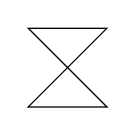
\begin{tikzpicture}
        \draw (0,0) -- (1,1) -- (0,1) -- (1,0) -- cycle;
    \end{tikzpicture}
    \caption{Какая-то хрень}\label{fig:1}
\end{figure}

\section{фф}

\section{фф}

\section{фф}

фф

\section{фф}

фф

\section{фф}

фф

\chapter{Основная часть}
Основная часть материала диссертации излагается в главах, в которых приводятся:

аналитический обзор литературы по теме~--– анализ работ, выполненных ранее отечественными и зарубежными исследователями, описание имеющихся подходов к исследованию проблемы, оценка степени изученности вопроса, формулирование проблемы, которая остается неразрешенной;

описание объектов исследования и используемых при проведении исследования методов, оборудования~--- характеристика основных подходов к решению поставленных задач, используемых теоретических и (или) экспериментальных методов и обоснование целесообразности их использования;

изложение выполненных в работе теоретических и (или) экспериментальных исследований.

Распределение основного материала магистерской диссертации по главам (разделам) и по параграфам (подразделам) определяются магистрантом. Весь порядок изложения в диссертации должен быть подчинен цели исследования, сформулированной автором. Дробление материала диссертации на главы, разделы, подразделы, а также их последовательность должны быть логически оправданными.

Каждую главу диссертации следует завершать краткими выводами.